\documentclass[aspectratio=169]{beamer}

\usepackage[utf8]{inputenc}
\usetheme{default}
\setbeamertemplate{navigation symbols}{}
\setbeamertemplate{footline}[frame number]

\title{dranspose: distributed event formation with dynamic map-reduce}
\author{Felix Engelmann \\\medskip \url{felix.engelmann@maxiv.lu.se}}
\date{30$^\text{th}$ November 2023}

\usepackage{tikz}
\usepackage{fontawesome5}

\DeclareFixedFont{\ttb}{T1}{txtt}{bx}{n}{12} % for bold
\DeclareFixedFont{\ttm}{T1}{txtt}{m}{n}{12}  % for normal

% Custom colors
\usepackage{color}
\definecolor{deepblue}{rgb}{0,0,0.5}
\definecolor{deepred}{rgb}{0.6,0,0}
\definecolor{deepgreen}{rgb}{0,0.5,0}

\usepackage{listings}

% Python style for highlighting
\newcommand\pythonstyle{\lstset{
language=Python,
basicstyle=\ttm,
morekeywords={self},              % Add keywords here
keywordstyle=\ttb\color{deepblue},
emph={EventData, StreamData,__init__},          % Custom highlighting
emphstyle=\ttb\color{deepred},    % Custom highlighting style
stringstyle=\color{deepgreen},
%frame=tb,                         % Any extra options here
showstringspaces=false
}}


% Python environment
\lstnewenvironment{python}[1][]
{
\pythonstyle
\lstset{#1}
}
{}

\begin{document}
\begin{frame}
\titlepage
\end{frame}

\begin{frame}{Existing Infrastructure}
\centering
 \begin{tikzpicture}
  \node at (-2,0) {Detectors};
  \node (det1) at (0,0) {\faCamera};
  \node (mot) at (4,0) {\faSlidersH}; %\faCameraRetro};
  \node (temp) at (6,0) {\faThermometerHalf};
  \node (det2) at (2,0) {\faVideo};
  
  \node at (-2,1) {Trigger Source};
  
  \node (panda) at (0,1) {\faWaveSquare};
  
  \draw[dotted] (panda) -- (det1);
  \draw[dotted] (panda) -- (det2.north);
  \draw[dotted] (panda) -- (mot.north);
  \draw[dotted] (panda) -- (temp.north);
  
  \node at (-2,-3) {File Recording};
  \node (file1) at (0,-3) {\faFileImage};
  \node (file2) at (2,-3) {\faFileImage};
  \node (file) at (5,-3) {\faFileArchive};
  
  \draw[very thick] (det1) -- (file1);
  \draw[very thick] (det2) -- (file2);
  
  \draw (mot) -- (file);
  \draw (temp) -- (file);
  
  \node at (-2,-2) {Live Analyses};
  \node (crop) at (0.5,-2) {\faCrop};
    
  \node at (-2,-4) {Post Analysis};
  \node (ana) at (3,-4) {\faChartArea};
  
  \draw (file1) -- (ana);
  \draw (file2) -- (ana);
  \draw (file) -- (ana);
  
  \node at (-2,-1) {Live Viewers};
  \node (live1) at (0.5,-1) {\faDesktop};
  \node (live2) at (2.5,-1) {\faDesktop};
  
  
  \draw (det2) -- (live2);
  
  \node (proc1) at (1.4,-2) {\faDesktop};
  \draw (det1) -- (live1) -- (crop) -- (proc1);
  
 \end{tikzpicture}

\end{frame}


\begin{frame}{Limitations of Live Analysis}
 \begin{block}{Single Data Stream}
  \begin{itemize}
   \item only one detector data available
   \item simple tools, e.g. azint, crop, time integration
   \item beyond limits: normalisation to $I_0$, sorting by motor position
  \end{itemize}
 \end{block}
 \begin{block}{Custom Modules}
  \begin{itemize}
   \item module development by SciDa
   \item custom deployment/integration
   \item custom live viewer interaction (mostly REST)
  \end{itemize}
 \end{block}
\end{frame}

\begin{frame}{Event Formation}
 \centering
 \begin{tikzpicture}
  \node at (-2,0) {Detectors};
  \node (det1) at (0,0) {\faCamera};
  \node (mot) at (4,0) {\faSlidersH}; %\faCameraRetro};
  \node (temp) at (6,0) {\faThermometerHalf};
  \node (det2) at (2,0) {\faVideo};
  
  \node at (-2,1) {Trigger Source};
  
  \node (panda) at (0,1) {\faWaveSquare};
  
  \draw[dotted] (panda) -- (det1);
  \draw[dotted] (panda) -- (det2.north);
  \draw[dotted] (panda) -- (mot.north);
  \draw[dotted] (panda) -- (temp.north);
  
  \node at (-2,-1) {Event Formation};
  \node (ef) at (3,-1) {\faHatWizard};
  
  \draw[very thick] (det1.south) -- (ef);
  \draw[very thick] (det2.south) -- (ef);
  \draw (mot.south) -- (ef);
  \draw (temp.south) -- (ef);
  
  
  \node at (-2,-2) {Analyses};
  \node (crop) at (3,-2) {\faCrop};
  
  \node (live) at (4,-2) {\faDesktop};
  
  \draw (crop) -- (live);
  
  \node at (-2,-3) {Reduced Recording};
  \node (file) at (3,-3) {\faFileArchive};
  \draw[line width=2mm] (ef) -- (crop);
  \draw[very thick] (crop) -- (file);
 \end{tikzpicture}
\end{frame}

\begin{frame}{Frame/Worker Matrix Transformation}
 \begin{minipage}[t]{0.49\textwidth}
 \begin{block}{Frame Stream}
 \medskip
  \begin{tabular}{rccccc}
   \faCamera & 1 & 2 & 3 & 4 & 5 \\
   \faVideo & 1 & 2  & 3 & 4 & 5\\
   \faSlidersH & 1 & & & 2 \\
   \faThermometerHalf & 1 & & 2 &  & 3 \\
  \end{tabular}
\end{block}
 \end{minipage}
 \begin{minipage}[t]{0.49\textwidth}
 \begin{block}{Event Stream}
 \medskip
    \begin{tabular}{rcccc}
     Event 1 & \faCamera\ 1 & \faVideo\ 1 &\faSlidersH\ 1 & \faThermometerHalf\ 1 \\
     Event 2 & \faCamera\ 2 & \faVideo\ 2 & & \\
     Event 3 & \faCamera\ 3 & \faVideo\ 3 & & \faThermometerHalf\ 2 \\
     Event 4 & \faCamera\ 4 & \faVideo\ 4 &\faSlidersH\ 2 &  \\
     Event 5 & \faCamera\ 5 & \faVideo\ 5 & & \faThermometerHalf\ 3 \\
    \end{tabular}
\end{block}
 \end{minipage}
 
 \begin{block}{Stream}
 \begin{itemize}
  \item matrix is sequentially filled column by column
  \item possibly unknown size (reactive scanning)
 \end{itemize}
 \end{block}


\end{frame}

\begin{frame}{Bandwidth and Latency}
 \begin{block}{Limitations}
  \begin{itemize}
   \item TCP connection max 60 Gbit/s
   \item ZMQ connection measured ca. 30 Gbit/s
  \end{itemize}
 \end{block}
 
 \begin{block}{Bottleneck}
 % \centering
 \begin{tikzpicture}
  \node at (1,-1) {Event Formation};
  \node (ef) at (3,-1) {\faHatWizard};
  
  \node at (1,-2) {Analyses};
  \node (crop) at (3,-2) {\faCrop};
  
  \draw[line width=2mm, color=title.fg] (ef) -- (crop);
 \end{tikzpicture}
 \end{block}
 
 \begin{block}{Processing Delay}
  \begin{itemize}
   \item acquisition at $\approx$ 100 -- 1000 Hz
   \item processing at $\approx$ 5-10 Hz
  \end{itemize}

 \end{block}
\end{frame}

\begin{frame}{Parallelisation}
 \centering
 \begin{tikzpicture}
  \node at (-2,0) {Detectors};
  \node (det1) at (0,0) {\faCamera};
  \node (mot) at (4,0) {\faSlidersH}; %\faCameraRetro};
  \node (temp) at (6,0) {\faThermometerHalf};
  \node (det2) at (2,0) {\faVideo};
  
  \node at (-2,1) {Trigger Source};
  
  \node (panda) at (0,1) {\faWaveSquare};
  
  \draw[dotted] (panda) -- (det1);
  \draw[dotted] (panda) -- (det2.north);
  \draw[dotted] (panda) -- (mot.north);
  \draw[dotted] (panda) -- (temp.north);
  
  \node at (-2,-1) {Event Formation};
  \node (ef1) at (0,-1) {\faHatWizard};
  \node (ef2) at (2,-1) {\faHatWizard};
  \node (ef) at (5,-1) {\faHatWizard};
  
  \draw[very thick] (det1.south) -- (ef1);
  \draw[very thick] (det2.south) -- (ef2);
  \draw (mot.south) -- (ef);
  \draw (temp.south) -- (ef);
  
  
  \node at (-2,-3) {Analyses};
  \node (crop1) at (0,-3) {\faCrop};
  \node (crop2) at (1,-3) {\faCrop};
  \node (crop3) at (2,-3) {\faCrop};
  \node (crop4) at (3,-3) {\faCrop};
  \node (crop5) at (4,-3) {\faCrop};
  \node (crop6) at (5,-3) {\faCrop};
  \node (crop7) at (6,-3) {\faCrop};
  
  \foreach \i in {1,2,...,7} {
    \draw (ef.south) -- (crop\i.north);
    \draw (ef1.south) -- (crop\i.north);
    \draw (ef2.south) -- (crop\i.north);
  };
  
 \end{tikzpicture}
 
 \begin{block}{Inter Event Analysis}
  \begin{itemize}
   \item time integration
   \item temporal correlations
  \end{itemize}

 \end{block}
\end{frame}

\begin{frame}{Sequential Reduce}
 \begin{block}{Operations at Acquisition Speed}
  \begin{itemize}
   \item append to list
   \item sum
  \end{itemize}

 \end{block}
 
 \centering
 \begin{tikzpicture}
  \node at (-2,-1) {Event Formation};
  \node (ef1) at (0,-1) {\faHatWizard};
  \node (ef2) at (2,-1) {\faHatWizard};
  \node (ef) at (5,-1) {\faHatWizard};
  
  \node at (-2,-2) {Analyses};
  \node (crop1) at (0,-2) {\faCrop};
  \node (crop2) at (1,-2) {\faCrop};
  \node (crop3) at (2,-2) {\faCrop};
  \node (crop4) at (3,-2) {\faCrop};
  \node (crop5) at (4,-2) {\faCrop};
  \node (crop6) at (5,-2) {\faCrop};
  \node (crop7) at (6,-2) {\faCrop};
  
  \node at (-2,-3) {Reduce};
  \node (red) at (3,-3) {\faCog};
  
  
  \foreach \i in {1,2,...,7} {
    \draw (ef.south) -- (crop\i.north);
    \draw (ef1.south) -- (crop\i.north);
    \draw (ef2.south) -- (crop\i.north);
    \draw (crop\i.south) -- (red);
  };
  
  \node (live) at (4,-3.5) {\faDesktop};
  \draw (red) -- (live);
  
  \node at (-2,-4) {Reduced Recording};
  \node (file) at (3,-4) {\faFileArchive};
  
  \draw[very thick] (red) -- (file);
  
  
 \end{tikzpicture}

\end{frame}

\begin{frame}{Intense Inter Event Computation}
\begin{minipage}{0.5\textwidth}

\begin{block}{Examples}
  \begin{itemize}
   \item aligning images (correlation)
   \item temporal fourier transform
  \end{itemize}
  
 \end{block}
 \begin{block}{Stateful Workers}
  \begin{itemize}
   \item load balance with constraints
   \item e.g. worker selected for event $n$ will also get $n+1$
  \end{itemize}

 \end{block}

\end{minipage}
\begin{minipage}{0.49\textwidth}
    \begin{tabular}{rcccc}
     \usebeamercolor[fg]{title} Worker 1 & \usebeamercolor[fg]{title} \faCamera\ 1 & \usebeamercolor[fg]{title} \faVideo\ 1 & \usebeamercolor[fg]{title}\faSlidersH\ 1 & \usebeamercolor[fg]{title} \faThermometerHalf\ 1 \\
     \usebeamercolor[fg]{title}Worker 1 & \usebeamercolor[fg]{title}\faCamera\ 2 &\usebeamercolor[fg]{title} \faVideo\ 2 & & \\
     Worker 2 & \faCamera\ 3 & \faVideo\ 3 & & \faThermometerHalf\ 2 \\
     Worker 2 & \faCamera\ 4 & \faVideo\ 4 &\faSlidersH\ 2 &  \\
     \usebeamercolor[fg]{title}Worker 1 & \usebeamercolor[fg]{title}\faCamera\ 5 &\usebeamercolor[fg]{title} \faVideo\ 5 & & \usebeamercolor[fg]{title}\faThermometerHalf\ 3 \\
    \end{tabular}
\end{minipage}

\end{frame}

\begin{frame}{Trigger Map}
 \begin{block}{Event Definitions}
  Which \emph{frames} from which \emph{detectors} belong to the same \emph{event} and have to be processed by the same \emph{worker}?
 \end{block}
    
\begin{block}{Virtual Workers}
\begin{itemize}
 \item virtual workers are dynamically assigned to real workers
 \item special \emph{all} workers (stream headers), or discard frame with $\emptyset$
 \item \emph{none} if stream has no frame for event
\end{itemize}

\medskip
 \begin{tabular}{rcccccc}
   \faCamera & all & 1 & 3 & 5 & 7 & 8 \\
   \faVideo & all & 2 & 4  & 6 & 7 & 9\\
   \faSlidersH & all & all & none & none & $\emptyset$ &none \\
   \faThermometerHalf & all & \{1,2\} & none & \{5,6\} & none  & \{8,9\} \\
  \end{tabular}
  \end{block}
  
  \begin{block}{Scanning}
   trigger map specified by scanning software, append-only extendable
  \end{block}

\end{frame}

\begin{frame}[fragile]{Development: Events}
 ease of use/development by SciDa and beamline staff
 
 \begin{block}{Event Structure}
  \begin{python}
StreamName = NewType("StreamName", str)
EventNumber = NewType("EventNumber", int)

class StreamData(BaseModel):
    typ: str
    frames: list[zmq.Frame]

class EventData(BaseModel):
    event_number: EventNumber
    streams: dict[StreamName, StreamData]

  \end{python}

 \end{block}

\end{frame}


\begin{frame}[fragile]{Development: Worker}
  \begin{python}
class FluorescenceWorker:
    def __init__(self):
        self.number = 0
    
    def process_event(self, event: EventData,
                      parameters=None):
        print(event)
        # parse zmq frames
        # fit spectra to get concentrations
        # extract motor position
        return {"position": mot, "concentrations": ...}
\end{python}
 
reinstantiated for every scan (new Trigger Map)
\end{frame}

\begin{frame}[fragile]{Development: Reducer}
 \begin{python}
class FluorescenceReducer:
    def __init__(self):
        self.publish = {"map": {}}
    
    def process_result(self, 
                      result: ResultData, 
                      parameters=None):
        print(result.event_number)
        print(result.worker)
        print(result.parameters_uuid)
        data = result.payload
        self.publish["map"][data["position"]] = \
                data["concentrations"]
\end{python}

reinstantiated for every scan (new Trigger Map)

\end{frame}

\begin{frame}[fragile]{Development: Viewer}
 \begin{block}{Jupyter Notebook}
  \begin{python}
import requests, pickle
import matplotlib.pyplot as plt

params = {}
requests.post("http://<ns>-ctrl.../params", json=params)
# start scan
r = requests.get("http://<ns>-reducer.../result/pickle")
data = pickle.loads(r.content)
# data = FluorescenceReducer.publish

plt.imshow(data["map"])
  \end{python}

 \end{block}

\end{frame}

\begin{frame}{Development: Silx based Viewer}
 \begin{block}{Parameters}
 \begin{itemize}
  \item set parameters
  \item influence slow processing
 \end{itemize}
 \end{block}

 \begin{block}{Partial Views}
  \begin{itemize}
   \item keep large accumulated data set on reducer
   \item query specific slice of \texttt{reducer.publish}
   \item e.g. \url{http://<ns>-reducer.../result/map/100:110,:}
  \end{itemize}
 \end{block}


\end{frame}


\begin{frame}{Development: Testing}
 \begin{block}{Recording}
  ingesters optionally write all zmq frames to disk (sequential pickle dumps)
 \end{block}
    
\begin{block}{Replay}
\begin{itemize}
 \item from recorded zmq frames
 \item from hdf5 files
\end{itemize}
\end{block}

\begin{block}{Local}
 run file-based ingesters, workers and reducer locally
\end{block}

\end{frame}

\begin{frame}
 \centering
 \Huge \usebeamercolor[fg]{title} Internals
\end{frame}

\begin{frame}{Architecture, ZMQ}
 \centering
 \begin{tikzpicture}[yscale=1]
  \node at (-2,1) {Detectors};
  \node (det1) at (0,1) {\faCamera};
  \node (mot) at (4,1) {\faSlidersH}; %\faCameraRetro};
  \node (temp) at (6,1) {\faThermometerHalf};
  \node (det2) at (2,1) {\faVideo};
  
  \node[color=title.fg, left] at (-1,0) {custom zmq};
  \node[color=title.fg, left] at (-1,-2) {wrapped(custom zmq)};
  \node[color=title.fg, left] at (-1,-4) {pickle in zmq};

  \node at (-2,-1) {Event Formation};
  \node (ef1) at (0,-1) {\faHatWizard};
  \node (ef2) at (2,-1) {\faHatWizard};
  \node (ef) at (5,-1) {\faHatWizard};
  
  \draw[very thick] (det1.south) --  (ef1);
  \draw[very thick] (det2.south) -- (ef2);
  \draw (mot.south) -- (ef);
  \draw (temp.south) -- (ef);
  
  
  \node at (-2,-3) {Analyses};
  \node (crop1) at (0,-3) {\faCrop};
  \node (crop4) at (3,-3) {\faCrop};
  \node (crop7) at (6,-3) {\faCrop};
  
  \foreach \i in {1,4,7} {
    \draw (ef.south) -- (crop\i.north);
    \draw (ef1.south) -- (crop\i.north);
    \draw (ef2.south) -- (crop\i.north);
  };
  
  \node at (-2,-5) {Reduce};
  \node (red) at (3,-5) {\faCog};
  
  
  \foreach \i in {1,4,7} {
    \draw (crop\i.south) -- (red.north);
  };
  
  \node[above of=ef2, yshift=-5mm, fill=white] {PULL};
  \node[above of=ef1, yshift=-5mm, fill=white] {PULL};
  \node[above of=ef, yshift=-5mm, fill=white] {SUB};
  
  \node[below of=det1, yshift=5mm, fill=white] {PUSH};
  \node[below of=det2, yshift=5mm, fill=white] {PUSH};
  \node[below of=mot, yshift=5mm, fill=white] {PUB};
  \node[below of=temp, yshift=5mm, fill=white] {PUB};
  
  \node[below of=ef1, yshift=5mm, fill=white] {ROUTER};
  \node[below of=ef2, yshift=5mm, fill=white] {ROUTER};
  \node[below of=ef, yshift=5mm, fill=white] {ROUTER};
  
  \node[above of=crop1, yshift=-5mm, fill=white] {\small DEALER};
  \node[above of=crop4, yshift=-5mm, fill=white] {\small DEALER};
  \node[above of=crop7, yshift=-5mm, fill=white] {\small DEALER};
  
  \node[below of=crop1, yshift=5mm, fill=white] {\small PUSH};
  \node[below of=crop4, yshift=5mm, fill=white] {\small PUSH};
  \node[below of=crop7, yshift=5mm, fill=white] {\small PUSH};
  
  \node[above of=red, yshift=-5mm, fill=white] {\small PULL};
 \end{tikzpicture}
\end{frame}

\begin{frame}{Architecture, redis}
 \begin{block}{\faDatabase\ config}
  \begin{itemize}
   \item components publish config (connected peers, trigger map version, zmq url)
   \item timeout for liveness probe
  \end{itemize}
 \end{block}
 
 \begin{block}{\faDatabase\ \faForward\ updates}
  \begin{itemize}
   \item controller notifies of new mapping/parameters
  \end{itemize}
 \end{block}
 
 \begin{block}{\faDatabase\ \faForward\ ready}
  \begin{itemize}
   \item workers notify readyness after event processed
  \end{itemize}
 \end{block}
 
 \begin{block}{\faDatabase\ \faForward\ assign}
  \begin{description}
   \item[event\_number:] EventNumber
   \item[assignments:] dict[StreamName, list[WorkerName]]
  \end{description}

 \end{block}

\end{frame}

\begin{frame}{Event Coordination}
\begin{block}{Controller}
\begin{itemize}
 \item wait for new entry in \faDatabase\ \faForward\ ready
 \item assign worker to first unassigned virtual worker (and \emph{all})
 \item distribute WorkAssignment in \faDatabase\ \faForward\ assign
\end{itemize}
\end{block}

\begin{minipage}[t]{0.49\textwidth}
 \begin{block}{Ingester}
  \begin{itemize}
   \item filter assignment for own streams
   \item combine all local streams
   \item copy event to specified workers (ROUTER)
  \end{itemize}

 \end{block}

\end{minipage}
\begin{minipage}[t]{0.49\textwidth}
 \begin{block}{Worker}
  \begin{itemize}
   \item filter assignment for own work
   \item listen to ingesters with participating streams
   \item assemble EventData
   \item call custom code
   \item send pickled result to reducer
   \item send ready message to \faDatabase\ \faForward\ ready
  \end{itemize}

 \end{block}

\end{minipage}

\end{frame}

\begin{frame}{Common Modules}
 \begin{block}{ZMQ Format / STINS}
  \begin{itemize}
   \item unpacking of (mulit-part) zmq frames to numpy arrays
  \end{itemize}
 \end{block}
 
  \begin{block}{Calibration}
\begin{itemize}
 \item installed as python modules
\end{itemize}
\end{block}

\begin{block}{Middlewares}
\medskip
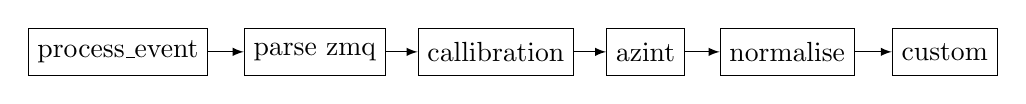
\begin{tikzpicture}
 \node[draw,minimum height=6mm] (proc) at (0,0) {process\_event};
 \node[draw,minimum height=6mm] (parse) at (2.5,0) {parse zmq};
 \node[draw,minimum height=6mm] (corr) at (4.8,0) {callibration};
 \node[draw,minimum height=6mm] (az) at (6.7,0) {azint};
 \node[draw,minimum height=6mm] (norm) at (8.5,0) {normalise};
 \node[draw,minimum height=6mm] (custom) at (10.5,0) {custom};
 \draw[-latex] (proc) -- (parse);
 \draw[-latex] (parse) -- (corr);
 \draw[-latex] (corr) -- (az);
 \draw[-latex] (az) -- (norm);
 \draw[-latex] (norm) -- (custom);
\end{tikzpicture}

\begin{itemize}
 \item maybe register required parameters?
 \item registered in Worker \texttt{\_\_init\_\_}
\end{itemize}


\end{block}
\end{frame}

\begin{frame}{Tests}
 \begin{block}{End-to-End}
  \begin{itemize}
   \item stream fake zmq frames
   \item full scan test
  \end{itemize}

 \end{block}
 \begin{block}{Protocols}
  \begin{itemize}
   \item Pydantic BaseModel (similar to dataclass)
   \item all messages defined and validated
   \item no \texttt{dict}s with random fields
  \end{itemize}
 \end{block}

\begin{block}{Typing}
 \begin{itemize}
 \item type hint annotations
  \item \texttt{mypy} strict
 \end{itemize}

\end{block}


\end{frame}

\begin{frame}{Deployment}
 \begin{block}{Docker}
  \begin{itemize}
   \item install custom dependencies
   \item end-to-end build latency multiple minutes
  \end{itemize}
 \end{block}
 
 \begin{block}{K8s}
  \begin{itemize}
   \item HELM chart for beamline
   \item restart pulls new version
   \item different containers for different experiments
  \end{itemize}
 \end{block}
    
\begin{block}{Versioning}
 \begin{itemize}
  \item add git commit hash to reduced data
  \item add parameters to h5 file
 \end{itemize}

\end{block}

\end{frame}

\begin{frame}{Performance}
 \begin{block}{Bandwidth}
  \begin{itemize}
   \item 10 Gbit/s from b-daq-cn2 and b-daq-cn3
   \item 8 workers
  \end{itemize}
 horizontally scalable if each stream $\leq$ 30 Gbit/s
 \end{block}
 
 \begin{block}{Latency}
  \begin{itemize}
   \item $\approx$ 2 kHz with enough workers
  \end{itemize}
  practically limited to $\approx n$  workers $\Rightarrow$ max worker runtime $\frac{n}{\text{acquisition rate [Hz]}}$s
 \end{block}
    \newcommand{\ev}{\mathsf{ev}}
    \newcommand{\st}{\mathsf{st}}
  \begin{block}{Virtual Worker Distribution}
  $\forall \st_0\in\mathbb{N}, h\in[|\mathsf{workers}|,\infty):$
   \[|\{M_{\ev,\st} : \st_0\leq\ev<(\st_0+h), \st\in\mathsf{streams}\}| > h-\epsilon \]
  \end{block}


\end{frame}




\begin{frame}{Outlook}
 \begin{block}{File Writing}
  \begin{itemize}
   \item custom by developers?
  \end{itemize}

 \end{block}
 
 \begin{block}{Autoscaling}
  \begin{itemize}
   \item observability of workers (queues)
   \item duty cycle of workers
   \item non-deterministic worker functions
   \item integration with k8s
  \end{itemize}

 \end{block}


 \begin{block}{Scan Integration}
  \begin{itemize}
   \item publish trigger map
   \item append to trigger map
  \end{itemize}

 \end{block}

\end{frame}


\end{document}
